\begin{definition} \textbf{Conjunto convexo.} \label{def:conjuntoconvexo}
    Sea $A \subseteq \Rn{n}$. Decimos que $A$ es un conjunto \emph{convexo} si para cualesquiera dos puntos $\vect{x}, \vect{y} \in A$, el segmento que los une está completamente contenido en $A$, es decir:
    \[
     \forall \vect{x}, \vect{y} \in A, \quad \lambda \vect{x} + (1 - \lambda)\vect{y} \in A \quad \forall \lambda \in \in [0,1].
    \]
\end{definition}

 \begin{center}
            \begin{minipage}{0.45\textwidth}
                \centering
                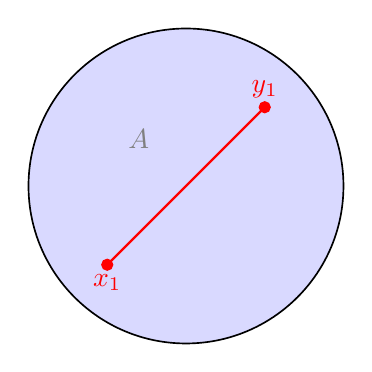
\begin{tikzpicture}
                    \draw[fill=blue!15, semithick] (0,0) circle(2);
                    \filldraw[red] (-1,-1) circle (2pt) node[below] {\(x_1\)};
                    \filldraw[red] (1,1) circle (2pt) node[above] {\(y_1\)};
                    \draw[thick, red, domain=-1:1] plot (\x, {\x});
                    \draw node at (-0.6,0.6) {\textcolor{gray}{$A$}};
                \end{tikzpicture}
            \end{minipage}
            \hspace{1cm} % espacio entre figuras
            \begin{minipage}{0.45\textwidth}
                \centering
                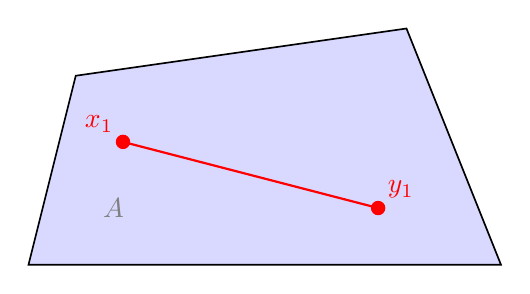
\begin{tikzpicture}[scale=1.2]
                    \filldraw[fill=blue!15, semithick] (-1.5,0) -- (3.5,0) -- (2.5,2.5) -- (-1,2) -- cycle;
                    \draw[thick, red] (-0.5,1.3) -- (2.2,0.6);
                    \filldraw[red] (-0.5,1.3) circle (2pt) node[above left] {\(x_1\)};
                    \filldraw[red] (2.2,0.6) circle (2pt) node[above right] {\(y_1\)};
                    \draw node at (-0.6,0.6) {\textcolor{gray}{$A$}};
                \end{tikzpicture}
            \end{minipage}
            \end{center}
            \begin{center}
            
\begin{tikzpicture}
                \node at (1.5,-2) {Conjuntos \emph{convexos}};
            \end{tikzpicture}
    
            \end{center}
            \begin{center}
                \begin{minipage}{0.45\textwidth}
                    \centering
                    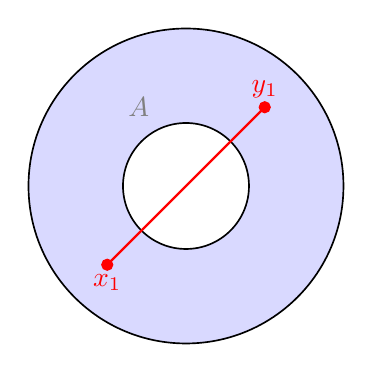
\begin{tikzpicture}
                        % Círculo exterior (azul claro) \draw[fill=blue!15, semithick] (0,0) circle(2);
                        \draw[fill=blue!15, semithick] (0,0) circle(2);
                        
                        % Círculo interior (blanco, para el hueco)
                        \draw[fill=white, semithick] (0,0) circle(0.8);
                        
                        \filldraw[red] (-1,-1) circle (2pt) node[below] {\(x_1\)};
                        \filldraw[red] (1,1) circle (2pt) node[above] {\(y_1\)};
                        \draw[thick, red, domain=-1:1] plot (\x, {\x});
                        
                        % Letra A
                        \draw node at (-0.6,1) {\textcolor{gray}{$A$}};
                    \end{tikzpicture}
                \end{minipage}
                \hspace{1cm} % espacio entre figuras
                \begin{minipage}{0.45\textwidth}
                    \centering
                    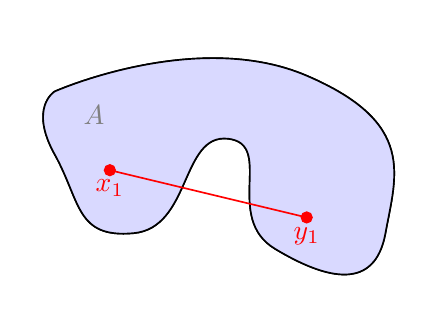
\begin{tikzpicture}
               
                        % Plane R^2 on the right
                       
                            \draw[semithick]
                                plot[smooth,tension=1.2] coordinates {(-0.2,0.8) (3,1) (4,-1) (2.6,-1.2)(2,0.2) (0.8,-1) (-0.2,0)(-0.2,0.8)};
                            
                            \filldraw[fill=blue!15, semithick]
                                plot[smooth, tension=1.2] coordinates {(-0.2,0.8) (3,1) (4,-1) (2.6,-1.2)(2,0.2) (0.8,-1) (-0.2,0)(-0.2,0.8)};
                                % \foreach \point in {(1,0.6), (3,0), (2.5,-1.5), (1,-1), (0.2,0.1), (1,0.6)} {
                                % \node at \point [circle,fill,inner sep=1pt] {};
                                % }
                                \filldraw[red] (0.5,-0.2) circle (2pt) node[below] {\(x_1\)};
                                \filldraw[red] (3,-0.8) circle (2pt) node[below] {\(y_1\)};
                                \draw[semithick, red] (0.5,-0.2) -- (3,-0.8); % Línea recta
                            \draw node at (0.3,0.5) {\textcolor{gray}{$A$}};
                            
                    
                    \end{tikzpicture}
                \end{minipage}
                \end{center}
                \begin{center}
                
\begin{tikzpicture}
                    \node at (1.5,-2) {Conjuntos \emph{arcoconexos y no convexos}};
                \end{tikzpicture}
                \end{center}
    
    